\section{Anwendung der Testgetriebenen Entwicklung}

In den nachfolgenden Abschnitten wird examplarisch an dem Objekt "`Job"', also einer Stellenanzeige, die Testgetriebene Entwicklung näher erläutert.
    
    
\subsection{Implementierung von Unit-Tests in Form von Modelltests}    

Ein Modell repräsentiert die Daten der Anwendung, und die Regeln, wie diese zu verändern sind. Bei Rails werden sie hauptsächlich dazu verwendet, um mit der zugrundeliegenden Datenbanktabelle zu interagieren. Per Konvention von Rails findet hier die Hauptarbeit, also die Business-Logik, statt.

Fast jeder Unittest bei Rails überprüft Validierungskritieren seines korrespondierenden Modells, d.h. wann eine Instanz dieses Modells gültig ist und damit gespeichert werden darf (man denke z.B. an Pflichtfelder für ein Modell "`Nutzer"` oder die Validierung des Formates seiner E-Mail-Adresse). Daneben sollten natürlich alle weiteren, selbstdefinierten, Methoden getestet werden.
% TODO http://guides.rubyonrails.org/getting_started.html#the-mvc-architecture

\paragraph{1. Der Anfang}
\begin{figure}[h]
 \centering
 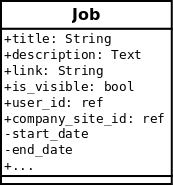
\includegraphics[width=0.3\textwidth]{../diagrams/job-erm.png}
 % job-erm.png: 173x186 pixel, 51dpi, 8.65x9.30 cm, bb=0 0 245 264
 \caption{Attribute des Modells "`Job"'}
  \label{fig:job-erm}
\end{figure}

Während der Analyse wurden die benötigten Attribute bestimmt. In Abbildung \ref{fig:job-erm} seien die Basisattribute der Tabelle dargestellt. Neben den einfachen Attributen, wie Title, Description und Link, existieren auch Referenzen auf andere Objekte (d.h. dies stellen Fremdschlüssel zu anderen Tabellen dar), wie z.B. Schlagwörter (Tags), ein Besitzer einer Stellenanzeige (User) und so weiter.


In der Regel erfolgt nun eine Generation der Testklasse und des Testmodells mittels der mitgelieferten Codegeneratoren. 
\begin{lstlisting}
~/it-jobs$ rails generate model job title:string link:string \
    description:text user:references visible:boolean ...

      invoke  active_record
      create    db/migrate/20110828160636_create_jobs.rb
      create    app/models/job.rb
      invoke    test_unit
      create      test/unit/job_test.rb
      create      test/fixtures/jobs.yml

\end{lstlisting}
Mit der Anweisung uns ein Modell "'job"` mit den nachfolgenden Attributen zu generieren, hat Rails uns nun schon ein Stück Arbeit abgenommen. Es wurden erstellt:
\begin{itemize}
 \item Eine Migration (\verb|db/migrate/2011xxxxxx_create_jobs.rb|). Dies stellt eine datenbankunabhängige Repräsentation einer Änderung an der Struktur unserer Datenbank dar. In diesem ist es die Erstellung einer Tabelle "'jobs"` (beachte: Plural!)
 \item Die Modelklasse (\verb|app/models/job.rb|)
 \item Die dazugehörige Testklasse (\verb|app/unit/job_test.rb|)
 \item und Fixtures-Datei (\verb|test/fixtures/jobs.yml|), zur Definition von Testdaten. 
\end{itemize}


Nach einer Erstellung der (SQLite)-Datenbank und Ausführung der Migration kann die Rails-Test-Suite nun auch schon ausgeführt werden:

\begin{lstlisting}
$ rake db:migrate && rake test
 
==  CreateJobs: migrating =====================================================
-- create_table(:jobs)
   -> 0.0020s
==  CreateJobs: migrated (0.0021s) ============================================

(in /home/zealot64/TEST)
Loaded suite /usr/lib/ruby/gems/1.8/gems/rake-0.8.7/lib/rake/rake_test_loader
Started
.
Finished in 0.043818 seconds.

1 tests, 1 assertions, 0 failures, 0 errors

\end{lstlisting}

Es wurde also schon ein Testfall erfolgreich ausgeführt, nämlich ein Dummytestfall von Rails:

\begin{lstlisting}
test/unit/job_test.rb 
require 'test_helper'

class JobTest < ActiveSupport::TestCase
  # Replace this with your real tests.
  test "the truth" do
    assert true
  end
end
\end{lstlisting}

\paragraph{2. Testen auf Validierung}

Ein Feature von Rails umfassen die sogenannten Validierungen. Diese stellen sicher, dass eine Instanz eines Modells nur dann gespeichert ist, wenn es gewissen Kritieren entspricht. Viele der Validations sind vergleichbar mit den Datenbank-Constraints einiger Datenbanken. Rails nutzt diese standardmäßig nicht, da es auch andere Persistenzsysteme unterstützt, wie z.B. Key-Value-Store, sogenannte NoSQL Datenbanken. So stellt Rails die Konsistenz und referenzielle Integrität innerhalb der Applikationsschicht sicher.

Nun möchten wir sicherstellen, dass eine Stellenanzeige nur dann gespeichert wird, wenn sie einen Titel beinhaltet. Der Test dazu würde wie folgt lauten:

\begin{lstlisting}
test/unit/job_test.rb 
require 'test_helper'

class JobTest < ActiveSupport::TestCase
  test "ein Job muss einen Titel haben" do
    job = Job.new
    job.title = nil
    assert !job.save
  end
end
\end{lstlisting}
Zuerst instanziieren wir einen Job, und geben ihm explizit einen leeren Titel, um das Testziel nochmal herauszustellen. Danach sichern wir zu, dass eine Speicherung nicht erfolgt, also "`false"' ist.

Nach Ausführung des Tests, schlägt dieser wie zu erwarten fehl.

Unser nächstes Ziel ist es nun, mit so wenig Code wie möglich den Test bestehen zu lassen. Das können wir mittels der eingebauten wie schon erwähnten Validierungen:

\begin{lstlisting}
class Job < ActiveRecord::Base
  validates :title, :presence => true
end
\end{lstlisting}

Nach erneuter Ausführung der Testsuite, besteht der Test nun. Jetzt folgt die Refaktorisierungsphase. Allerdings lässt sich der Programmcode, nicht weiter vereinfachen. Allerdings ist der Testcode ausdrücklich nicht von Refaktorisierungen befreit, und könnten z.B. so ansetzen.

\begin{lstlisting}
test "ein Job muss einen Titel haben" do
  job = Job.new :title => nil
  assert !job.save
end
\end{lstlisting}



Nun wollen wir dasselbe für das Feld E-Mail tun, hierbei aber nicht nur das Vorhandensein prüfen, sondern auch das Format.

\begin{lstlisting}
test "ein Job muss eine gültige E-Mail haben" do
  job = Job.new :email => "invalid_email"
  assert !job.save
end
\end{lstlisting}
Die Implementierung wäre dann:
\begin{lstlisting}
class Job < ActiveRecord::Base
  validates :email, :format => /^[\w\d_\-]+@[\w\d_\-]\.[\w\d]{2,3}$/
  ...
\end{lstlisting}

\paragraph{3. Refaktorisierungen der Testklasse}

Nun fehlt aber noch ein positiv-Beispiel für einen gültigen Job zu definieren:

\begin{lstlisting}
test "ein Job muss einen Titel haben" do
  job = Job.new :title => "Rails Entwickler", :email => "info@stefanwienert.net"
  assert_valid job
end
\end{lstlisting}
Dieser Test besteht sofort, macht also genau genommen keine weitere Aussage über unser System. Nach der "`reinen"' Testgetriebenen Leere sollte dieser entfernt werden. Es ist allerdings eine gute Strategie, bei Validierungen mindestens ein Beispiel zu präsentieren, dass angenommen wird. Nichtsdestotrotz können wir nun Refaktorisieren. Insbesondere unsere Testfunktionen enthalten unnötige Redundanzien:

\begin{lstlisting}
test "ein Job muss einen Titel haben" do
  job = Job.new :title => nil
  assert !job.save
end
test "ein Job muss eine gültige E-Mail haben" do
  job = Job.new :email => "invalid_email"
  assert !job.save
end
test "ein Job muss einen Titel haben" do
  job = Job.new :title => "Rails Entwickler", :email => "info@stefanwienert.net"
  assert_valid job
end
\end{lstlisting}
In allen drei Methoden wird ein Job instanziiert, und lediglich verschiedene Attribute überprüft. Auch haben unsere ersten beiden Tests keine gültige Aussage mehr, da der jeweilige Job sowieso nicht gültig ist, da jeweils das andere Attribut fehlt\footnote{Im ersten Test ist nicht nur der Titel nicht gesetzt, sondern auch die E-Mail entspricht nicht dem Format}. Es ist also höchste Zeit, die Tests zu refaktorisieren. Dies geschieht am Besten durch die Verwendung einer Testdaten-Generation, z.B. den eingebauten Fixtures, die Rails uns bei der Codegeneration schon mit generiert hatte. Dabei definieren wir zentralisiert unsere (gültigen) Testdaten, die von Rails vor jedem einzelnen Test in der Datenbank bereitgestellt werden:

\begin{lstlisting}
# test/fixtures/jobs.yml
valid_job:
  title: Rails Entwickler
  email: info@stefanwienert.net
  link: http://www.example.com/jobs
  visible: true
  ...
invisible_job:
  title: Rails Entwickler
  visible: false
  ...
  
  
\end{lstlisting}

Nun können wir diese Fixtures in unseren Tests verwenden, und das ganze in einer setup-Methode, die vor jedem Testfall aufgerufen wird, laden:
\begin{lstlisting}
setup do
  @job = jobs :valid_job
  # Dies lädt den Job mit dem Schlüssel "valid_job"
  #  und schreibt ihn in die Instanzvariable @job
  #  der Testklasse 
end

test "stelle sicher, dass die Fixtures valide sind" do
  assert_valid @job
end
test "ein Job muss einen Titel haben" do
  @job.title = nil
  assert !@job.save
end
test "ein Job muss eine gültige E-Mail haben" do
  @job.email = "invalid_email"
  assert !@job.save
end
\end{lstlisting}
Am Ende dieser Refaktorisierungen ist es notwendig, die Tests noch einmal auszuführen.
Danach würde die Implementierung einer nächsten Teilanforderung sein. Was in diesem Abschnitt zu sehen war ist, dass die Testgetriebene Entwicklung das Arbeiten und Testen in kleinen Schritten favorisiert.

\subsection{Implementierung von Controller-Tests (functional tests)}

Neben den Unittests stellt Ruby on Rails eine weitere Testart nativ bereit. Technisch gesehen handelt es sich bei diesen Functional Tests aber auch um Unittests, da deren Testobjekt ein Controller ist. 
Ein Controller hat bei Ruby on Rails die Aufgabe, Anfragen für bestimmte Routen, also Web-Adressen, anzunehmen, die Arbeit an eine Modelklasse auszulagern, und eine View aufzurufen, die letztendlich HTML-Code generiert.

Im ersten Beispiel wollen wir testen, dass ein Gast-Nutzer, also z.B. ein Bewerber, eine sichtbare Stellenanzeige aufrufen darf (visible = true). Hierbei verwenden wir wieder unser oben definiertes Fixture für einen gültigen Job.
\begin{lstlisting}
/test/functional/jobs_controller_test.rb 
require 'test_helper'

class JobsControllerTest < ActionController::TestCase
  test "Gast Nutzer kann Stellen betrachten" do
    session[:user_id] = nil
    job = jobs(:valid_job)
    
    get :show, :id => job.id
    
    assert_response :success
    assert_equal job, assigns(:job)
  end
end
\end{lstlisting}
Zuerst loggen wir jeglichen Nutzer aus, der eventuell eingeloggt war, dann laden wir das Fixture und führen einen simulierten HTTP Request auf die Detailansicht der Stellenanzeige aus (Die Aktion "`show"' mit der ID des Jobs).
Nun erwarten wir, dass wir einen HTTP-Status Code 200 (success) erhalten, und dass der Controller eine Variable "`@jobs"' bereitstellt, die mit unserem Fixture identisch ist.

Die Implementation dieser Anforderung könnte wie folgt umgesetzt werden:
\begin{lstlisting}
# app/controllers/jobs_controller.rb
class JobsController < ApplicationController
  ...
  def show
    @job = Job.first
  end
  ...
  
end
\end{lstlisting}
Das Laden des erstem Jobs aus unserer Datenbank genügt zum Erfüllen der Anforderungen, und ist ein schneller Weg, den Test bestehen zu lassen. Allerdings handelt es sich hierbei um eine Fake-Implementierung, da zwar unser Test erfüllt wird, aber die Anwendung nicht das macht, was man sich erhofft hat. Solche Zwischenschritte sind aber ausdrücklich vorgesehen, da das Ziel ist, so schnell wir möglich einen funktionierenden Test zu erhalten mit dem man arbeiten kann.

Wenn wir nun weitere Tests schreiben, so wird es immer schwieriger, die Fake-Implementierung beizubehalten, und früher oder später wird eine korrekte Implementierung folgen. 
Aber wir können auch die nun folgende Refaktorisierungsphase nutzen, um diesen Makel zu beseitigen:
\begin{lstlisting}
# app/controllers/jobs_controller.rb
def show
  @job = Job.find(params[:id])
end
\end{lstlisting}

Nun wollen wir testen, ob ein Gast von einer nicht-sichtbaren Stellenanzeige weitergeleitet wird und einen Hinweis erhält.
\begin{lstlisting}
test "Gast Nutzer kann nicht-sichtbare Stellen nicht betrachten" do
  session[:user_id] = nil
  job = jobs(:invisible_job)
  
  get :show, :id => job.id

  assert_response :redirect
  assert flash[:notice].present?
end
\end{lstlisting}
Wir laden unser zweites definiertes Fixture, dass eine unsichtbaren Stellenanzeige. Dieses mal erwarten wir einen HTTP Statuscode 301 (Redirect), und dass unser Controller eine Hinweisnachricht generiert.

\begin{lstlisting}
def show
  @job = Job.find(params[:id])
  if not @job.visible?
    redirect_to root_path, :notice => "Diese Stelle ist zur Zeit nicht sichtbar"
  end
end
\end{lstlisting}
Falls der aktuelle Job nicht sichtbar ist, dann erfolgt eine Weiterleitung auf die Startseite und die Bereitstellung des Hinweistextes.

Da auch hier der Quelltext wieder sehr kurz ist, ist ein Refaktorisieren nicht notwendig.

Nun möchten wir, dass ein Kunde dieser Anwendung, also ein Unternehmen seine Stellenanzeige betrachten kann, auch wenn diese unsichtbar ist, sei es aus Gründen der Archivierung als auch der Vorbereitung für eine Veröffentlichung.
\begin{lstlisting}
test "Ein Kunde darf aber seine unsichtbaren Jobs betrachten" do
  job = jobs(:invisible_job)
  session[:user_id] = job.user_id
  
  get :show, :id => job.id

  assert_response :success
end
\end{lstlisting}
Über die globale Session Variable simulieren wir das Einloggen durch setzen der UserID in dieses Array. Die genaue Implementation hängt natürlich davon ab, wie man die Authentifizierung implementiert hat, oder welche Bibliothek man verwendet. In diesem Beispiel sei darauf hingewiesen, dass die Definition, ob ein Nutzer eingeloggt ist oder nicht, davon abhängt, ob in seiner Session-Variable eine UserID enthalten ist.

\begin{lstlisting}
def show
  @job = Job.find(params[:id])
  if !@job.visible? and @job.user != User.find(session[:user_id])
    redirect_to root_path, :notice => "Diese Stelle ist zur Zeit nicht sichtbar"
  end
end
\end{lstlisting}
Wir lösen diesen Test damit, dass wir in der Weiterleitungsbedingung prüfen, ob der betrachtende Nutzer und der Eigentümer des Jobs gleich sind.

Nun können wir refaktorisieren. Was auffällt, ist z.B. dass unser Controller und die Klasse Job nicht lose gekoppelt sind, da die Bedingung zweimal auf Attribute des Jobs zurückgreift. Eine Lösung wäre die Auslagerung in die Modelklasse von Job:
\begin{lstlisting}
# app/models/job.rb
class Job < ActiveRecord::Base
  ...
  def visible_for_user?(user)
    self.visible and self.user != user
  end 
end

# app/controllers/jobs_controller.rb 
def show
  @job = Job.find(params[:id])
  unless @job.visible_for_user?(User.find(session[:user_id]))
    redirect_to root_path, :notice => "Diese Stelle ist zur Zeit nicht sichtbar"
  end
end
\end{lstlisting}
Ebenfalls wurde das syntaktische Element "`unless"' verwendet, welches ein sprechbares "`if not"' ist.
Weiterhin könnte die Suche nach dem aktuell eingeloggten Nutzer in eine für alle Controller sichtbare Funktion ausgegliedert werden

\begin{lstlisting}

# app/controllers/application_controller.rb
...
  def current_user
    User.find(session[:user_id]
  end

# app/controllers/jobs_controller.rb 
def show
  @job = Job.find(params[:id])
  unless @job.visible_for_user? current_user
    redirect_to root_path, :notice => "Diese Stelle ist zur Zeit nicht sichtbar"
  end
end
\end{lstlisting}



\subsection{Testen von externen Abhängigkeiten}
 mittels Mocks und Stubs am Beispiel Feedimport

\subsection{System und Akzeptanztests}


\subsection{Testen von Javascript Ereignissen}
\subsubsection{Test im Rahmen von Integrationstest}
Systemtests mittels Selenium fuer vereinzeltes JS in Form von

\subsubsection{Unittests mit Javascript}
Unittests:  Jasmine fuer komplexe Objekte und Javascript Anwendungen






